\section{Auswertung}

\subsection{Strahlenschutzmessung}

In Aufgabe 1 nahmen wir Messungen bezüglich des Strahlenschutzes vor. Dazu verwendeten wir ein mobiles Dosimeter und nahmen die aus Tabelle \ref{dft:Arbeitsplatz} bekannten Messdaten an verschiedenen Orten auf. Zur besseren Verdeutlichung, wo wir gemessen haben, folgt eine Skizze des Labors.

\vspace{5mm}

\begin{center}
    \minipanf    
        \makebox[\textwidth]{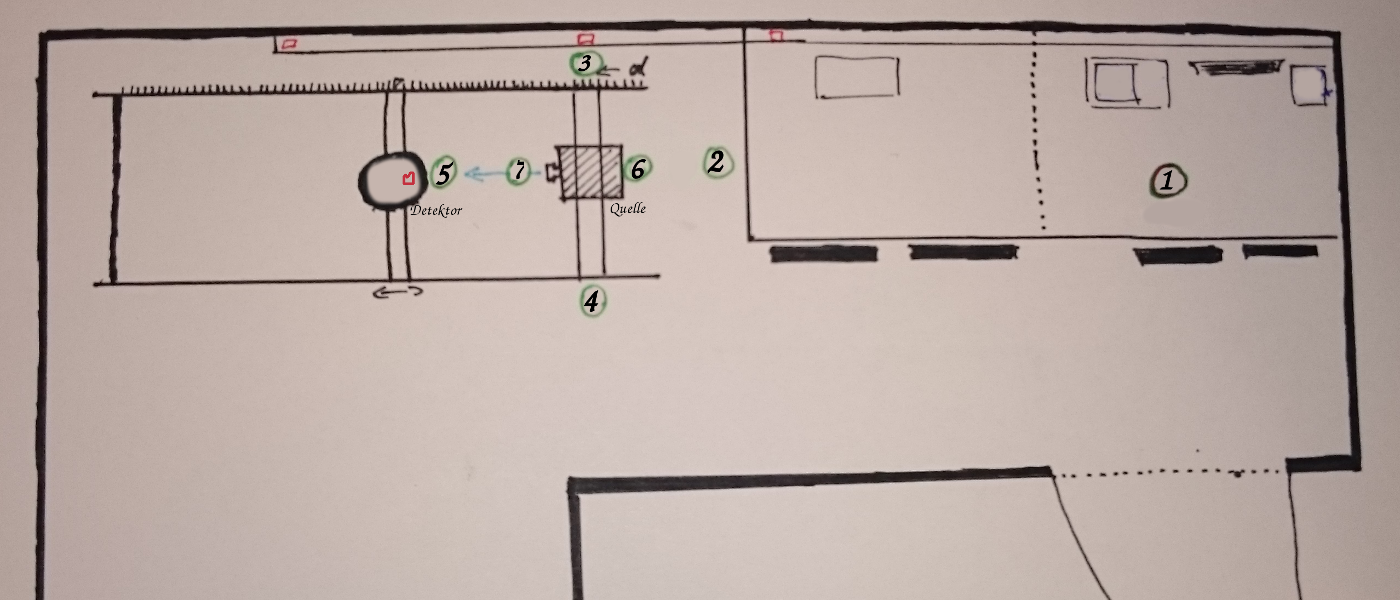
\includegraphics[width=1.4\linewidth, height=0.4\textheight]{pic/skizze}}
        \captionof{figure}{Raumskizze zu Messorten (nicht maßstabsgerecht)\\ 
                            \textbf{1:} Arbeitsplatz, \textbf{2:} 50cm hinter Quelle, \textbf{3:} 50cm rechts der Quelle, \textbf{4:} 50cm links, \textbf{5:} 50cm davor, \textbf{6:} 8cm dahinter, \textbf{7:} 8cm davor}
        \label{fig:skizze}
    \minipend
\end{center}

\vspace{5mm}

Die roten Kästchen im Bild bezeichnen die vier Punkte, an denen die BeO-Detektoren lagen. Die oberen drei liegen auf einer Steckerleiste, ca. 40cm unterhalb der Quelle. Das Kästchen bei \textbf{5} bezeichnet den \textquotedblleft Mitfahrer \textquotedblright.

\subsubsection{Strahlungswerte im Labor am Anfang des Versuchstages}

Schauen wir uns nun interessante Orte an. Tabelle \ref{dft:Arbeitsplatz} zeigt deutlich, dass am PC-Arbeitsplatz kein Risiko besteht, die 6mSv, die ein Praktikant oder Auszubildender im Jahr nicht überschreiten darf, zu erreichen. Nähert man sich der Quelle auf 50cm an und bleibt dahinter stehen, so verringert sich offenbar die maximale Aufenthaltsdauer pro Tag. Offenbar ist ein achtstündiger Arbeitstag noch immer in der Maximaldauer von 21 Stunden enthalten. \\
Jetzt wird es interessanter. Links und rechts von der Quelle, scheint die Abschirmung des Kollimators nicht mehr so stark wie hinter der Quelle. Ein Arbeitstag darf von einem Praktikanten also nicht daneben verbracht werden, sondern, unter Berücksichtigung der Fehler, die man während der Messung durch Zittrigkeit erzeugt, höchsten 7 Stunden - pro Tag, 7 Tage die Woche. 
In der Strahlrichtung vor der Quelle misst man erwartungsgemäß deutlich höhere Dosen, die die maximale Verweildauer pro Tag minimieren. 8cm vor der verschlossenen Kollimatoröffnung sollte man sich als Student möglichst weniger als 20 Minuten aufhalten.\\
Deutlich wird auch, dass die Belastung durch Strahlung überall um die Quelle größer wird, wenn man den Kollimatorverschluss öffnet. So haben wir hinter dem Kollimator zwar immer noch fast zwei Arbeitstage, um die Eintagesagesdosis zu erreichen, verlieren aber in Zahlen sechst Stunden an Aufenthaltsdauer. \\
Dabei ist zu beachten, dass die Tagesdosis den ganzen Tag betrifft, also 24 Stunden.
Die Maximaldauer ergibt sich aus der durchschnittlichen Tagesdosis folgendermaßen:

\begin{equation*}
    t_{max} = \frac{0,0164 mSv}{\dot D} 
\end{equation*}
\ \\
Dabei trägt \.D die Einheit mSv/h\\

Bezüglich der Messergegbnisse kann man noch weitere Fehlerquellen erwähnen. Das verwendete Dosimeter  ist nicht nur einer Unsicherheit durch den Haltenden ausgesetzt, sondern wurde auch bemerkt, dass zu verschiedenen Zeitpunkten die Messwerte sprungartig in die Höhe schnellten und sich nach ca. zwei Minuten senkten, was in etwa der Zeit für die Mittelung des Gerätes entspricht.

\subsubsection{Strahlendosis im Labor über 2 Tage}
Nun schauen wir uns Tabelle \ref{dft:Raum} an. Hier wurden Daten über fast zwei Tage gesammelt. Man sieht 
deutlich, dass der Mitfahrer, welcher am Versuchstag immer schwankenden Werten ausgesetzt war, eine Dosis von 
etwa 0,5mSv gemessen hat. Dies entspricht etwa der Hälfte von dem, was eine Standardperson in einem Jahr an 
künstlicher Strahlenzufuhr erfahren darf. Fraglich ist allerdings, ob dieser Wert nicht ein Ergebnis von Störungen, 
die andere Experimente verursacht haben, ist, da auch mit dem tragbaren Dosimeter zwischenzeitlich einzelne Peaks gemessen wurden.
Man erkennt allerdings gut, dass der BeO-Sensor, der hinter der Quelle lag, eine deutlich geringere Strahlendosis maß als jene, die auf der Steckerleiste 1,8m vor und auf der Steckerleiste neben der Quelle lagen. Dies bestätigt die Vermutung, die Abschirmung hinter der Quelle sei stärker als jene an den Seiten.


\subsection{Abstandsquadratgesetz}
Wir haben durch unsere Messung mit dem Beo\textit{max}-System das Abstandsquadratgesetz bestätigt. Dafür haben wir die Werte aus Tabelle \ref{dft:Abstandsquadrat} geplottet und einen Fit der Form $\dot{D} = c/(d-d_0)^2$ gemacht, welcher unter Betrachtung der Fehlerintervalle sehr gut passt. Da die am Boden befindliche Messskala, an der wir den Abstand $d$ abgelesen haben, bündig mit der Öffnung des Kollimators begonnen hat, die Quelle sich aber tatsächlich in einem Abstand $d' = d + d_0$ vom Messpunkt befand, haben wir den zusätzlichen Verschiebungsparameter $d_0$ eingeführt, um zusätzlich die wahre Position der Quelle zu bestimmen.

	\minipanf    
        \makebox[\textwidth]{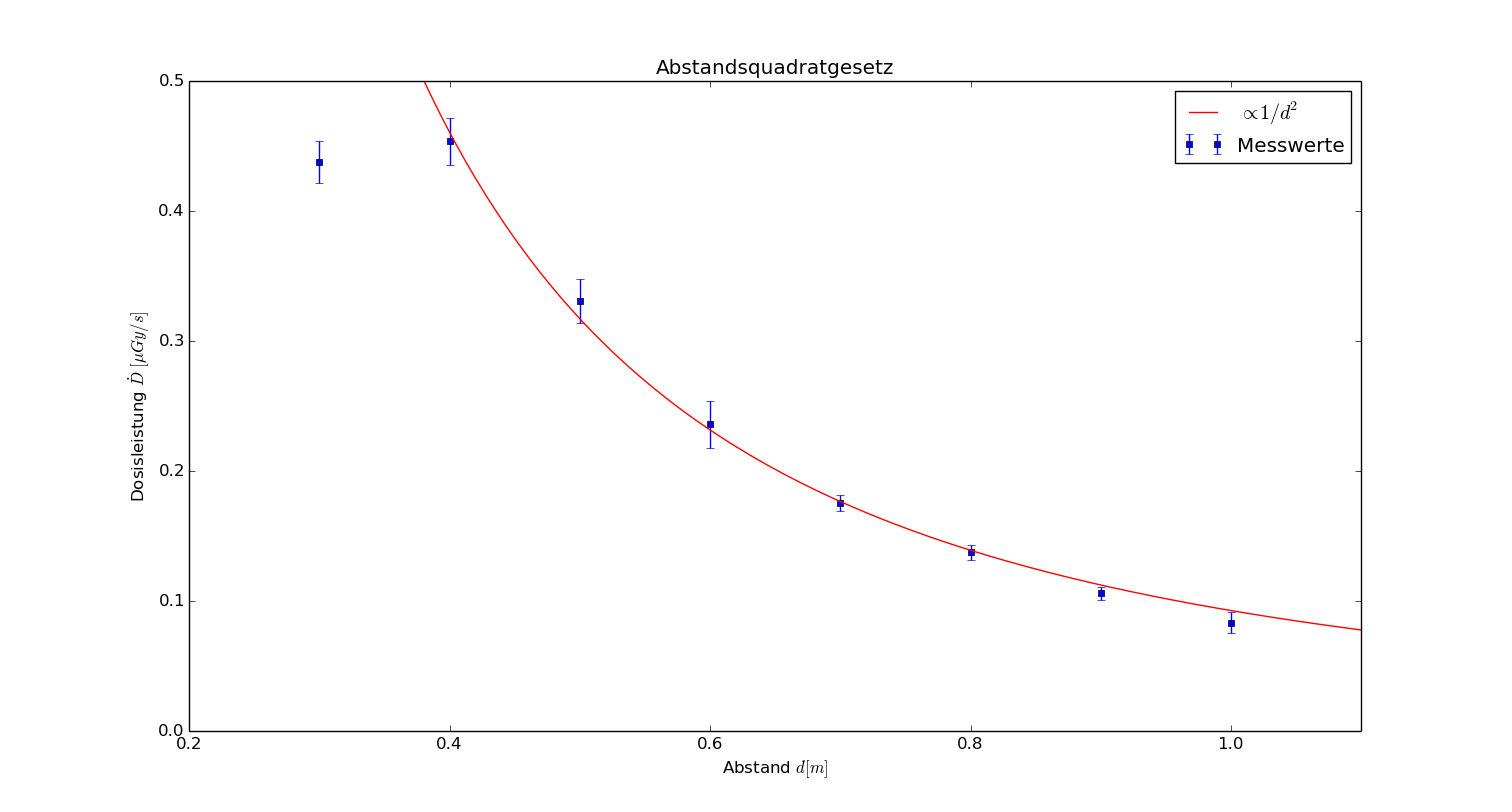
\includegraphics[width=1.2\linewidth, height=0.4\textheight]{pic/abstandsquadratgesetz}}
        \captionof{figure}{Bestätigung des Abstandsquadratgesetzes}
        \label{fig:Abstandsquadrat}
    \minipend
    \vspace{5mm}

Wir haben die Fit-Parameter, und somit die wahre Position der Quelle, (mit ihren Standardabweichungen) wiefolgt bestimmt:
\begin{equation*}
		c = (0.109 \pm 0.008)\ \mu Gy \cdot m^2/s
\end{equation*}
\begin{equation*}
		d_0 = (0.087 \pm 0.019) m
\end{equation*}

Dabei ist anzumerken, dass wir den Messwert für $d=0,2\ m$ beim Fitten nicht mit einbezogen haben, da sich dieser - vermutlich aufgrund einer zu kurzen Bestrahlungszeit - nicht gut in die anderen Messwerte einreiht.

\subsection{Winkelabhängigkeit der kollimierten Quelle}
Wir haben in Tabelle \ref{dft:Aufweitung} den Zusammenhang zwischen dem transversalem Abstand zur Öffnung des Kollimators und der Dosisleistung bestimmt. Folgende Graphik veranschaulicht unsere Ergebnisse:

    \minipanf    
		\begin{center}    
        	 \makebox[\textwidth]{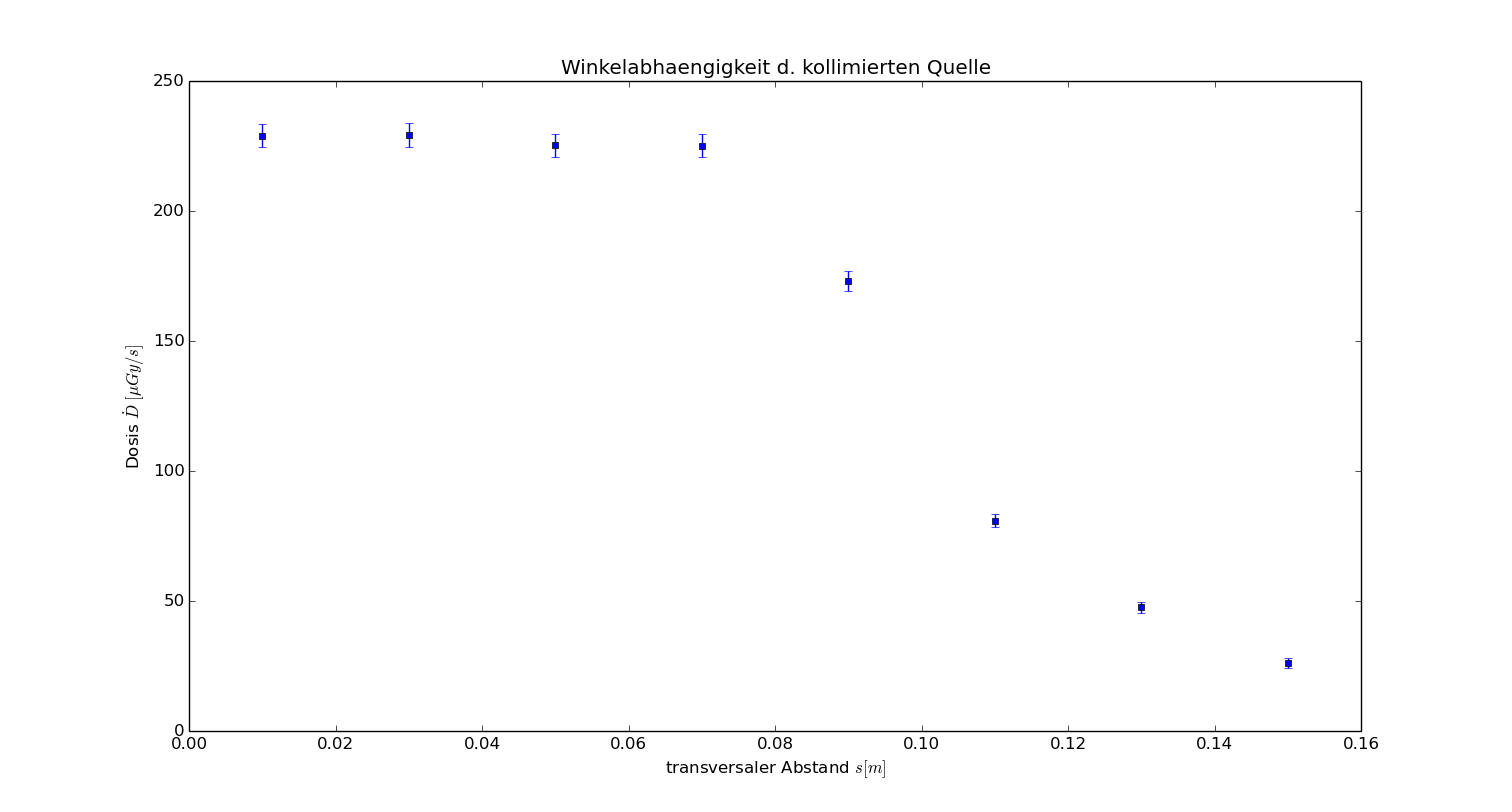
\includegraphics[width=1.2\linewidth,
        	 height=0.4\textheight]{pic/winkelabhaengigkeit}}
       		 \captionof{figure}{Aufweitung der kollimierten Quelle}
        \label{fig:Aufweitung}
        \end{center}
    \minipend
    \vspace{5mm}

Man sieht, dass sich die Dosisleistung bis zu einem Abstand $d=0.07\ m$ nicht ändert, da dies der Bereich ist, auf dem die aus der Kollimatoröffnung austretenden Photonen entweder direkt oder durch Beugung an der Öffnung auftreffen. Für größere Abstände fällt die Dosis - wie erwartet - rapide ab, da dann ausschließlich wenige gebeugte oder reflektierte Photonen in diese Bereiche geraten beziehungsweise die meisten $\gamma$-Quanten durch die Abschirmung gestoppt werden.
